\documentclass{article}
\usepackage[utf8]{inputenc}
\usepackage{physics}
\usepackage{listings}
\usepackage{graphicx}
\usepackage{flexisym}

\title{Applied Mathematics TW324 Assignment 04}
\author{Bhekimpilo Ndhlela (18998712)}

\date{13 April 2018}
\begin{document}
\maketitle
\pagebreak
\section*{Question 1}
\subsection*{Python Source Code For Both a.) and b.): }
\begin{lstlisting}[language=Python]
def question_a(steps, x=0.0, debug=False):
    fp = lambda x, h : ((-f(x+2*h)+8*f(x+h)-8*f(x-h)+f(x-2*h))/(12*h))
    f = lambda x : sqrt(1 - 2 * sin(x))
    exact = [abs(fp(x, h) + 1.0) for h in steps]
    if debug is True:
        print "DEBUG MODE: [ON] QUESTION 1 a.)"
        print "i","\t" ,"Step Size", "\t", "Exact Error"
        for i, (h, err) in enumerate(zip(steps, exact)):
            print (i+1), "\t","{:.7f}".format(h), "\t", "{:.10f}".format(err)
    return exact

def question_b(steps, M=11.0, debug=False):
    machine_eps = finfo(float).eps
    bound = [(18.0 * machine_eps)/(12.0*h) + M*(h**4) for h in steps]
    if debug is True:
        print "DEBUG MODE: [ON] QUESTION 3 bii.)"
        print "i","\t" ,"Step Size", "\t", "Bound"
        for i, (h, err) in enumerate(zip(steps, bound)):
            print (i+1), "\t","{:.7f}".format(h), "\t", "{:.10f}".format(err)
    return bound

def plot_err_functs(steps, exact, bound):
    #loglog plot to display the error as function of the step size
    plt.title("Plot of the Exact Error and Bound as h(Step size) Changes")
    plt.xlabel("h (Step Size)")
    plt.ylabel("Exact vs Bound")
    plt.yscale('log')
    plt.xscale('log')
    plt.plot(steps, exact, "k-", label="Exact")
    plt.plot(steps, bound, "k--", label="Bound")
    plt.legend(bbox_to_anchor=(.65, .9))
    plt.show()

if __name__ == "__main__":
    from numpy import (abs, cos, sin, sqrt, logspace)
    from numpy import (finfo, float)
    import matplotlib.pyplot as plt
    from math import pow

    steps = logspace(-7, -1, num=100)
    exact, bound = question_a(steps), question_b(steps)
    plot_err_functs(steps, exact, bound)
\end{lstlisting}
\pagebreak
\begin{figure}[h!]
  \centering
  \begin{subfigure}{\linewidth}
    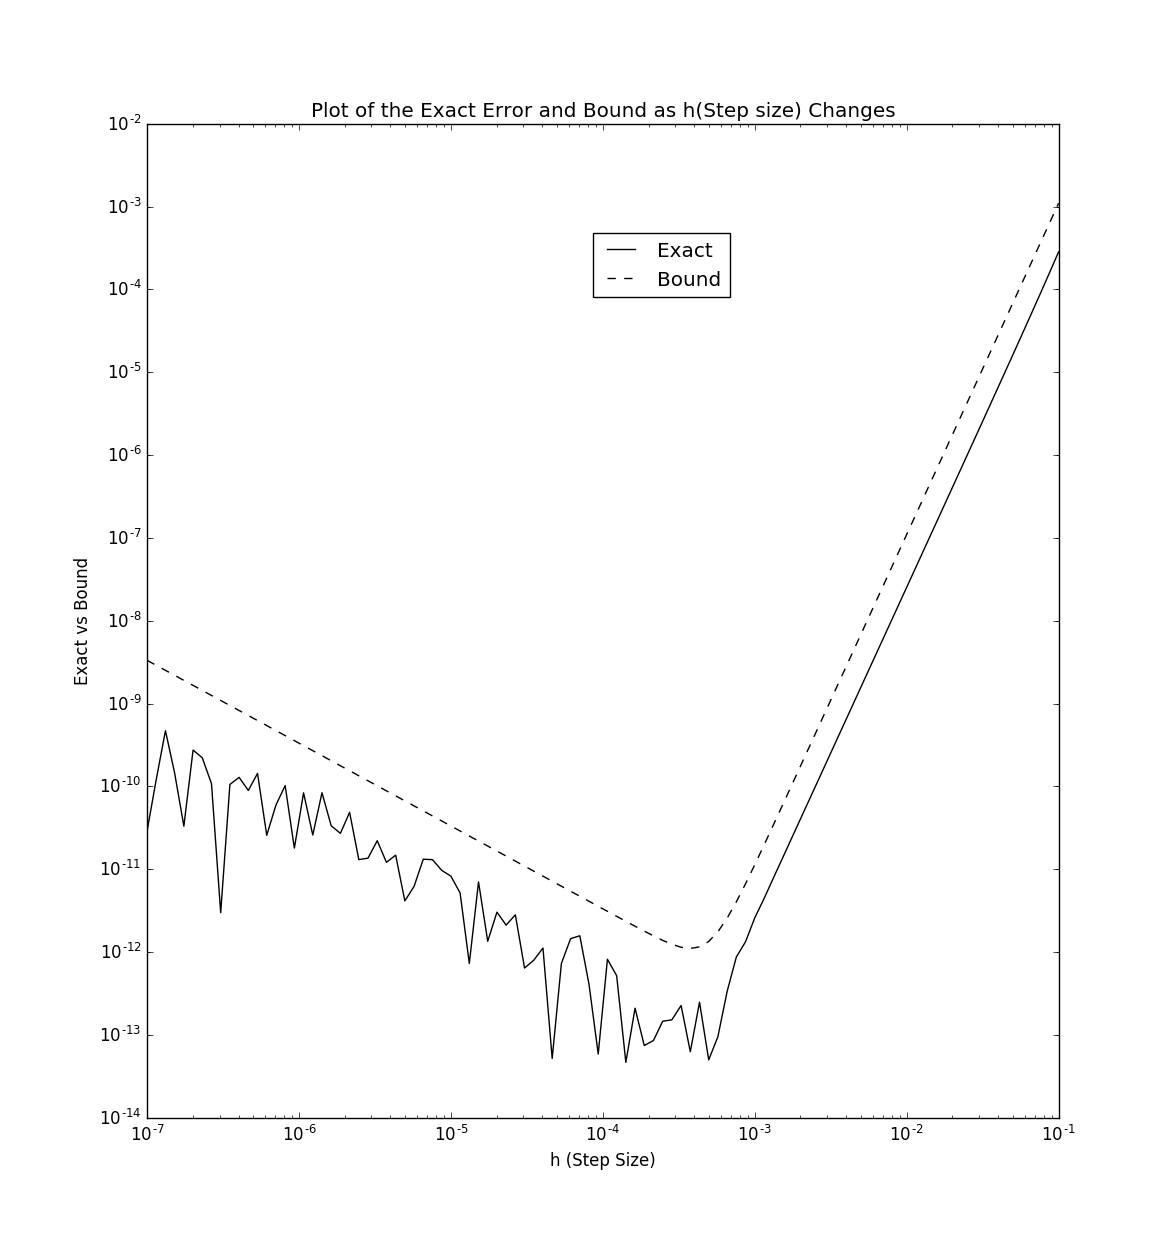
\includegraphics[width=\linewidth]{question1a_b.png}
    \caption{approximation of the first derivative of $f(x)$ with the error bound}
  \end{subfigure}
\end{figure}
\textbf{Conclusion: The conclusion matchs the O(h^4) convergence predicted by the theory?}
\pagebreak



\pagebreak
\section*{Question 2}
\textbf{Required To Prove That: $\int_{a}^{b} x^3 dx = \frac{h}{3}(y_0 + 4y_1 + y_2) - \frac{h^5}{90} f^{(iv)}(c)$ \\ \\}
\textbf{We Know That The Exact Integral is: $\int_{a}^{b}x^3 dx = \frac{1}{4}x^4 |_{a}^{b} = \frac{1}{4}(b^4 - a^4)$\\ \\  The Simpson's Rule States That:\\ \\ }
\textbf{$\int_{x_0}^{x_2} x^3 dx = \frac{h}{3}(y_0 + 4y_1 + y_2) - \frac{h^5}{90} f^{(iv)}(c) $ \\ \\ but: $y_0 = a^3 $, $y_2 = b^3$ and $y_1 = (\frac{a + b}{2})^3$ also: $ -\frac{h^5}{90} f^{(iv)}(c) = 0$ because:\\ \\ 
$f(x) = x^3$, $f{\prime}(x) = 3x^2$, $f{\prime \prime}(x) = 6x$, $f^{(iiv)}(x) = 6$ and $f^{(iv)}(x) = 0  $ \\ \\ we also know that: $h = \frac{b - a}{2} \implies \frac{h}{3} = \frac{b - a}{6}$ Then:\\ \\}
\begin{align*}
    \int_{a}^{b}f(x)dx &= \frac{b - a}{6}(b^3 + 4(\frac{a + b}{2})^3 + a^3) \\
    \int_{a}^{b}f(x)dx &= \frac{b - a}{6}(b^3 + 4(\frac{a^3 +3a^2b + 3ab^2 + b^3}{8}) + a^3)\\
    \int_{a}^{b}f(x)dx &= \frac{b - a}{6}(b^3 + (\frac{a^3 +3a^2b + 3ab^2 + b^3}{2}) + a^3) \\
    \int_{a}^{b}f(x)dx &= \frac{b - a}{6}(\frac{2b^3 + b^3 + a^3 + 3a^2b + 3ab^2 + 2a^3}{2})\\
    \int_{a}^{b}f(x)dx &= \frac{b - a}{6}(\frac{3b^3 +3a^2b + 3ab^2 + 3a^3}{2})\\
    \int_{a}^{b}f(x)dx &= \frac{(b - a)(3b^3 +2a^2b + 2ab^2 + 3a^3)}{12})\\
    \int_{a}^{b}f(x)dx &= \frac{(b - a)(3b^3 +2a^2b + 2ab^2 + 3a^3)}{12})\\
    \int_{a}^{b}f(x)dx &= \frac{3b^4 - 3a^4}{12}\\
    \int_{a}^{b}f(x)dx &= \frac{3(b^4 - a^4)}{12}\\
    \int_{a}^{b}f(x)dx &= \frac{1}{4}(b^4 - a^4)
\end{align*}
\textbf{Conclusion: Since $\int_{a}^{b}f(x)dx$ (Exact Solution) $ = \int_{a}^{b}f(x)dx$ (Simpsons Method) then I have proved that the Simpson’s rule has polynomial degree of precision since i have shown  exact for the integral}

\pagebreak
\section*{Question 3}
\subsection*{a.)}

\textbf{Required To Prove: \\ $f{\prime \prime}(x) = \frac{-f(x - 2h) + 16f(x + h) - 30f(x) + 16f(x - h) - f(x - 2h)}{12h^2} + O(h^4)$\\  by the aid of Extrapolation\\ \\ \\ }
\textbf{Consider Case 1: use $h$ \\ \\ 
$f{\prime \prime}(x) = \frac{f(x + h) - 2f(x) + f(x - h)}{h^2} - \frac{h^2}{12}f^{(iiv)}(c) + O(h^4)$ \\ \\}
\textbf{Consider Case 2: use $2h$ \\ \\ $f{\prime \prime}(x) = \frac{f(x + 2h) - 2f(x) + f(x - 2h)}{4h^2} - \frac{4h^2}{12}f^{(iiV)}(c) + O(h^4)$ \\ \\ now we use: $4*$case $1$ - case $2$ \\ \\ }
\textbf{$4f{\prime \prime}(x) - f{\prime \prime}(x) = \frac{4f(x + h) - 8f(x) + 4f(x - h)}{h^2} - \frac{4h^2}{12}f^{(iiv)}(c) + O(h^4) - ( \frac{f(x+2h) - 2f(x) + f(x-2h)}{4h^2}+ \frac{4h^2}{12}f^{(iiv)}(c) + O(h^4))$\\ \\ $3f{\prime \prime}(x) = \frac{16f(x + h) - 32f(x) + 16f(x-h) - f(x +2h) - 2f(x) - f(x - 2h)}{4h^2} + O(h^4)$ \\ \\ \\ $f{\prime \prime}(x) = \frac{-f(x-2h) + 16f(x+h) - 30f(x) + 16f(x-h) - f(x-2h)}{12h^2} + O(h^4)$ \\ \\ \\ I have used the method of extrapolation to derive the second derivative approximation}



\pagebreak
\subsection*{b.)}
\subsection*{Python Source Code For: }
\begin{lstlisting}[language=Python]
def exact(steps, x=0.0, debug=False):
    fpp = lambda x, h : ((-f(x+2*h)+16*f(x+h)-30*f(x)+16*f(x-h)-f(x-2*h))\
                                           /(12*h*h))
    f = lambda x : sqrt(1 - 2 * sin(x))
    exact = [abs(fpp(x, h) + 1.0) for h in steps]
    if debug is True:
        print "DEBUG MODE: [ON] QUESTION 3 bi.)"
        print "i","\t" ,"Step Size", "\t", "Exact Error"
        for i, (h, err) in enumerate(zip(steps, exact)):
            print (i+1), "\t","{:.7f}".format(h), "\t", "{:.10f}".format(err)
    return exact

def bound(steps, M=11.0, debug=False):
    machine_eps = finfo(float).eps
    bound = [(18.0 * machine_eps)/(12.0*(h**2)) + M*(h**4) for h in steps]
    if debug is True:
        print "DEBUG MODE: [ON] QUESTION 3 bii.)"
        print "i","\t" ,"Step Size", "\t", "Bound"
        for i, (h, err) in enumerate(zip(steps, bound)):
            print (i+1), "\t","{:.7f}".format(h), "\t", "{:.10f}".format(err)
    return bound

def plot_error_functions(steps, exact, bound):
    #loglog plot to display the error as function of the step size
    plt.title("Plot of the Exact Error and Bound as h(Step size) Changes")
    plt.xlabel("h (Step Size)"); plt.ylabel("Exact vs Bound")
    plt.yscale('log'); plt.xscale('log')
    plt.plot(steps, exact, "k-", label="Exact")
    plt.plot(steps, bound, "k--", label="Bound")
    plt.legend(bbox_to_anchor=(.65, .9))
    plt.show()

if __name__ == "__main__":
    from numpy import (abs, cos, sin, sqrt, logspace)
    from numpy import (finfo, float)
    import matplotlib.pyplot as plt
    from math import pow

    steps = logspace(-7, -1, num=100)
    exact, bound = exact(steps), bound(steps)
    plot_error_functions(steps, exact, bound)
\end{lstlisting}
\pagebreak
\begin{figure}[h!]
  \centering
  \begin{subfigure}{\linewidth}
    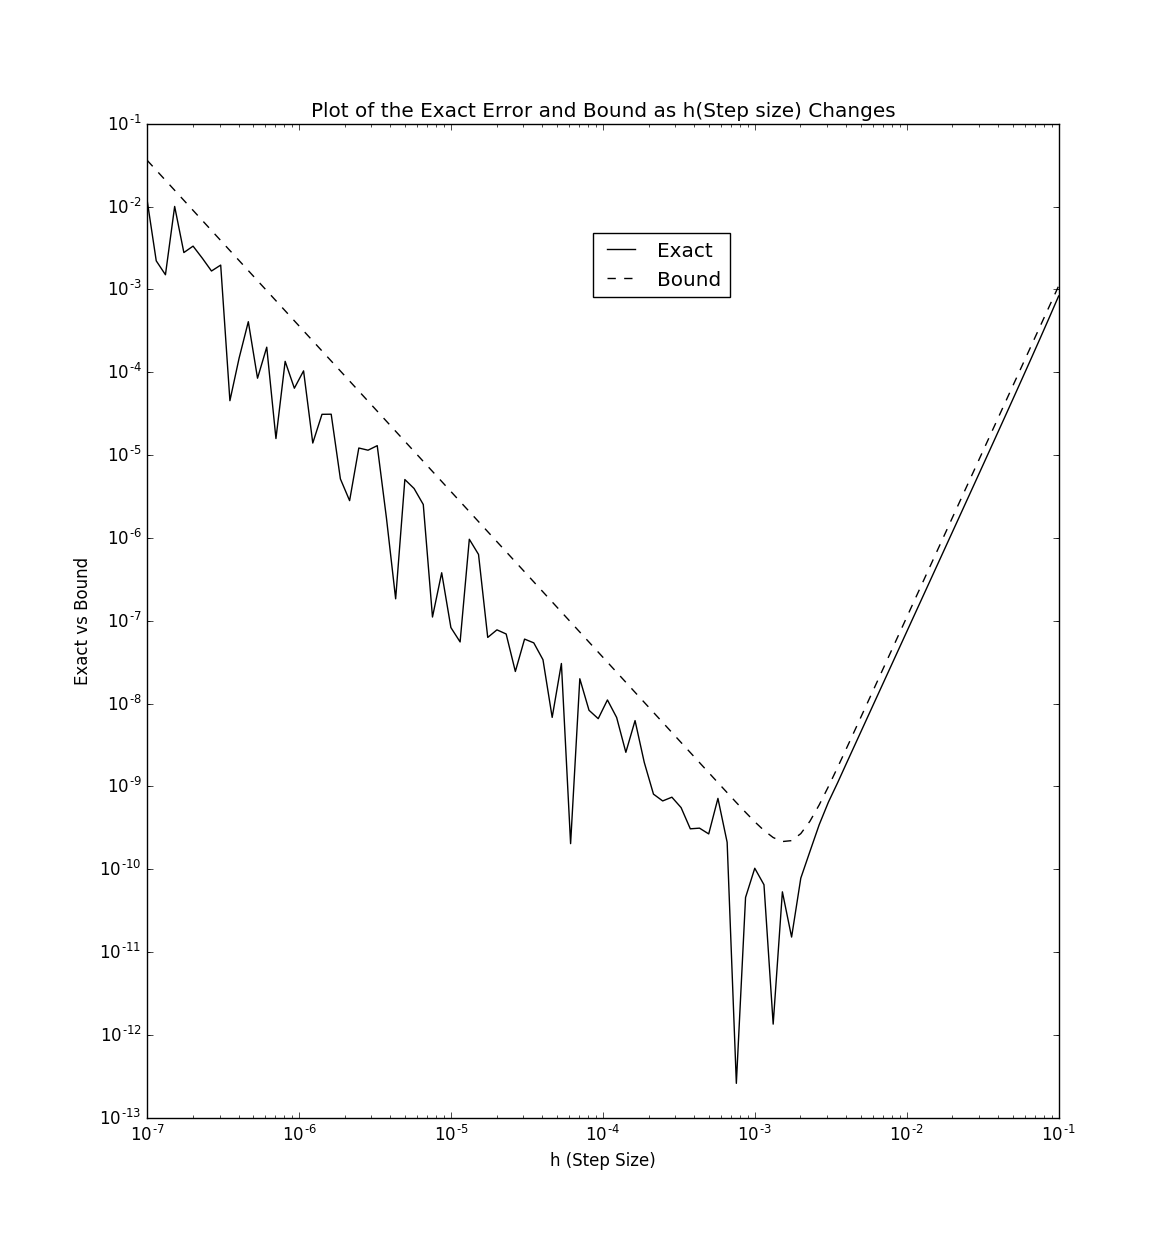
\includegraphics[width=\linewidth]{question3b.png}
    \caption{approximation of the second derivative of $f(x)$ from Question 1(a) with the error bound of $f(x)$}
  \end{subfigure}
\end{figure}
\textbf{Conclusion: The conclusion matches the O(h^4) convergence predicted by the theory?}
\pagebreak


\section*{Question 4}
\subsection*{Python Source Code: }
\begin{lstlisting}[language=Python]
def trapezium(exact_I, H, x0=0., debug=True):
    apprx_I = array([h/2. * (exp(x0) + exp(h)) for h in H])
    return array([abs(apI - exI) for apI, exI in zip(apprx_I, exact_I)])

def midpoint(exact_I, H, x0=0., debug=True):
    W = array([x0 + (h / 2.0) for h in H])
    apprx_I = array([h * exp(w) for h, w in zip(H, W)])
    return array([abs(apI - exI) for apI, exI in zip(apprx_I, exact_I)])

def simpson(exact_I, H, x0=0., debug=True):
    apprx_I = array([h/6.*(exp(x0)+(4.*exp(h/2.))+exp(h)) for h in H])
    return array([abs(apI - exI) for apI, exI in zip(apprx_I, exact_I)])

def debug(abs_err_s, abs_err_m, abs_err_t, debug=True):
    if debug is True:
        print "DEBUG MODE: [ON] [Question 4 Simpson's method]"
        print "SIMPSONS METHOD\t\tMIDPOINT METHOD\t\tTRAPEZIUM METHOD"
        for s, m, t in zip(abs_err_s, abs_err_m, abs_err_t):
            print "{:.20f}".format(s),"{:.20f}".format(m),"{:.20f}".format(t)
    else:
        print "DEBUG MODE: [OFF] [Question 4 Simpson's method]"

def plot_abs_errs(abs_err_t, abs_err_m, abs_err_s):
    #loglog plot to display the error as function of the step size
    plt.title("|xc-x| of: The Midpoint, Simpson & Trapezium Methods against h")
    plt.ylabel("Midpoint vs Simpson vs Trapezium")
    plt.xlabel("h"); plt.yscale('log'); plt.xscale('log')
    plt.plot([1., .1, .01], abs_err_t, "k-", label="Trapezium")
    plt.plot([1., .1, .01], abs_err_m, "r-", label="Midpoint")
    plt.plot([1., .1, .01], abs_err_s, "g-", label="Simpson")
    plt.legend(bbox_to_anchor=(.65, .9))
    plt.show()

if __name__ == "__main__":
    from numpy import (exp, abs, array)
    import matplotlib.pyplot as plt
    H, exact_I = array([1., .1, .01]), array([exp(h) - 1 for h in H])
    abs_err_t = trapezium(exact_I, H)
    abs_err_m = midpoint(exact_I, H)
    abs_err_s = simpson(exact_I, H)
    debug(abs_err_s, abs_err_m, abs_err_t)
    plot_abs_errs(abs_err_t, abs_err_m, abs_err_s)
\end{lstlisting}

\begin{center}
    \begin{tabular}{||c| c|| c||} 
    \hline
    \textbf{SIMPSONS METHOD} & \textbf{MIDPOINT METHOD} & \textbf{TRAPEZIUM METHOD}\\ [0.5ex] 
    \hline\hline
    0.00057932341754773908 & 0.06956055775891689663 & 0.14085908577047745460\\ [1ex] 
    \hline
    0.00000000365068135444 & 0.00004380843804530077 & 0.00008762782813467873\\ [1ex] 
    \hline
    0.00000000000003500325 & 0.00000004187557393898 & 0.00000008375125289117\\ [1ex] 
    \hline
    \end{tabular}
\end{center}

\begin{figure}[h!]
  \centering
  \begin{subfigure}{\linewidth}
    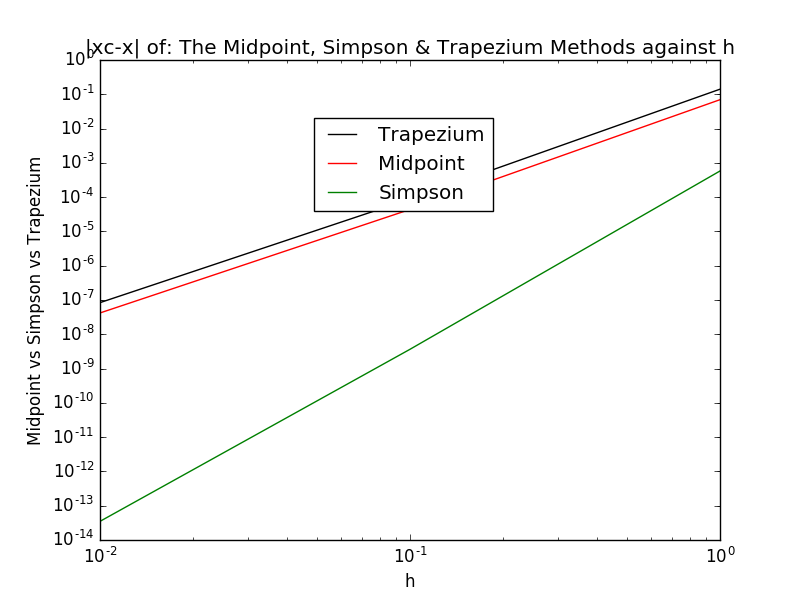
\includegraphics[width=\linewidth]{question4.png}
    \caption{$|x_c - x|$Absolute Errors for the SIMPSONS, MIDPOINT and the TRAPEZIUM METHOD }
  \end{subfigure}
\end{figure}
\textbf{\\ \\ \\Conclusion: The rates of convergence agree with the theoretical
approximations derived in lectures}




\pagebreak
\section*{Question 5}
\subsection*{Python Source Code: }
\begin{lstlisting}[language=Python]
def question_a(n=8.0, debug=True):
    h = (1.0 / (n - 1.0))
    f = array([exp(x) for x in linspace(0.0, 1.0, 8.0)])
    A = matrix([[1,-2, 1, 0, 0, 0, 0, 0],\
                [0, 1,-2, 1, 0, 0, 0, 0],\
                [0, 0, 1,-2, 1, 0, 0, 0],\
                [0, 0, 0, 1,-2, 1, 0, 0],\
                [0, 0, 0, 0, 1,-2, 1, 0],\
                [0, 0, 0, 0, 0, 1,-2, 1]])
    f_ = (1.0 / h**2.0) * matmul(A, f).T

    if debug is True:
        print "DEBUG MODE: [ON] \t [QUESTION 5 A.)]"
        print "f\"(x) = ",
        for i in f_:
            print i,

if __name__ == "__main__":
    from numpy import (linspace, exp, array, shape, matrix, matmul)
    import matplotlib.pyplot as plt
    question_a()
\end{lstlisting}

\begin{center}
    \textbf{Answer/ Result: \\ \\ \\ }
\end{center}

\begin{center}
\textbf{ $f^{\prime \prime}(x)$ = \begin{bmatrix}1.15552818 \\1.33297685 \\1.53767544\\1.77380856\\2.04620346\\2.36042868 \end{bmatrix}}
\end{center}
\pagebreak

\end{document}


